\documentclass[10pt,twocolumn]{article}
	
\usepackage{myfontstyle}
\usepackage{mypackages}
\usepackage{mymacros}
\usepackage{mycommands}

\begin{document}
\thispagestyle{fancy1}

%%% Title and Abstract------------------------
\twocolumn[
\begin{center}
	\hrule
	\vspace{3pt}
	% Title:
	{\sffamily\bfseries\Large
		Report for Laboratory Two: Voltage Dividers
	} \\
	{\color{gray}
		\vspace{3pt}
		\hrule
		\vspace{3pt}
	}
	{
		\hspace*{\fill}
		Austin Piper
		\hspace*{\fill}
		Alex Blakely
		\hspace*{\fill}
		Irfan Ahmed
		\hspace*{\fill}
%		Fourth Author    % uncomment these two lines if there's a fourth author
%		\hspace*{\fill}
	}\\
	\vspace{3pt}
	{\itshape
		\hspace*{\fill}
		Department of Mechanical Engineering, Saint Martin's University
		\hspace*{\fill} \\
		\hspace*{\fill}
		ME/EE 316---Mechatronics \& Measurements Laboratory
		\hspace*{\fill}
	}\\
	\vspace{3pt}
	{
		\hspace*{\fill}
		\today{} % today's date ... can type manually instead
		\hspace*{\fill}
	}
	\vspace{3pt}
	{\color{gray}\hrule}
%	\vspace{2pt}
\end{center}
% Abstract:
\begin{adjustwidth}{1.5in}{1.5in}
{\small
\noindent\textbf{Abstract.} \hspace{1em}
	Applying a 10V DC power supply to a voltage divider circuit with two resistors in series, the voltage across both resistors remains constant while the voltage across a single resistor changes depending on the resistance. Using a myRIO configured with the labVIEW software to change our input voltage and measure the voltage source and the resistor voltage. When connecting an arbitrary function generator to an oscilloscope, a variety of wave functions at 5Vpp had a period of 2.5ms.
}
\end{adjustwidth}
\vspace{9pt}
\hrule
\vspace{1\baselineskip}
]

%%% Body -------------------------


\section{Introduction} 
\label{sec:introduction}

The voltage divider (shown in figure \ref{fig:circuit}) is a fundamental electronic circuit that allows an input voltage to be split into different output voltages using resistors. The output of such a circuit is described by equation \ref{eq:2}.\\
The purpose of this lab is to better understand the voltage divider circuit, as well as the concepts of voltage and signal generation (as well as measurement). While observing the effects of different resistors on the output voltage, the team gained experience with using the myRIO in conjuction with a computer for realtime circuit measurements. The latter portion of the lab also enabled the team to use an oscilloscope to observe the qualities of a function supplied by a function generator.

\section{Materials and Methods}

	This lab has three parts. In the first part of the lab two resistors were placed in series on a bread board connected to a DC power supply set to 10V. A multimeter was used measure the voltage across each resistor and both resistors and the data was recorded. After the resistance is measured, the second resistor in the series is replaced by another resistor of a higher strength, taking measurements again for all four different resistors. The goal is to find how the voltage differs across the circuit compared to across the resistors when source voltage is held constant and the resistance is varied.\autoref{fig:circuit}
	
	
	For part two of this lab a myRIO configured with the labVIEW software was be used as the power supply and measurement tool on the same voltage divider circuit. The myRIO was connected to measure the voltage across both resistors and the voltage across the second resistor. Using labVIEW an analog output and input were made to recieve data from the myRIO, as well as a voltage vs time chart window. Starting at 0V and working up to 10V, in increments of 1V, the voltage source and the resistor voltage is displayed in labVIEW and recorded. The second resistor in the series is, again, replaced with each of the different resistors and the voltage across the resistors is measured once again.\autoref{fig:myrio} 
	

	In part three of this lab an arbitrary function generator was connected to an oscilloscope. While producing a sine wave with the function generator set to 5Vpp, then by adjusting the oscilloscope settings a stable wave was found and the peak to peak amplitude and period were estimated.\autoref{fig:stable}
	
\begin{figure}
	\centering
	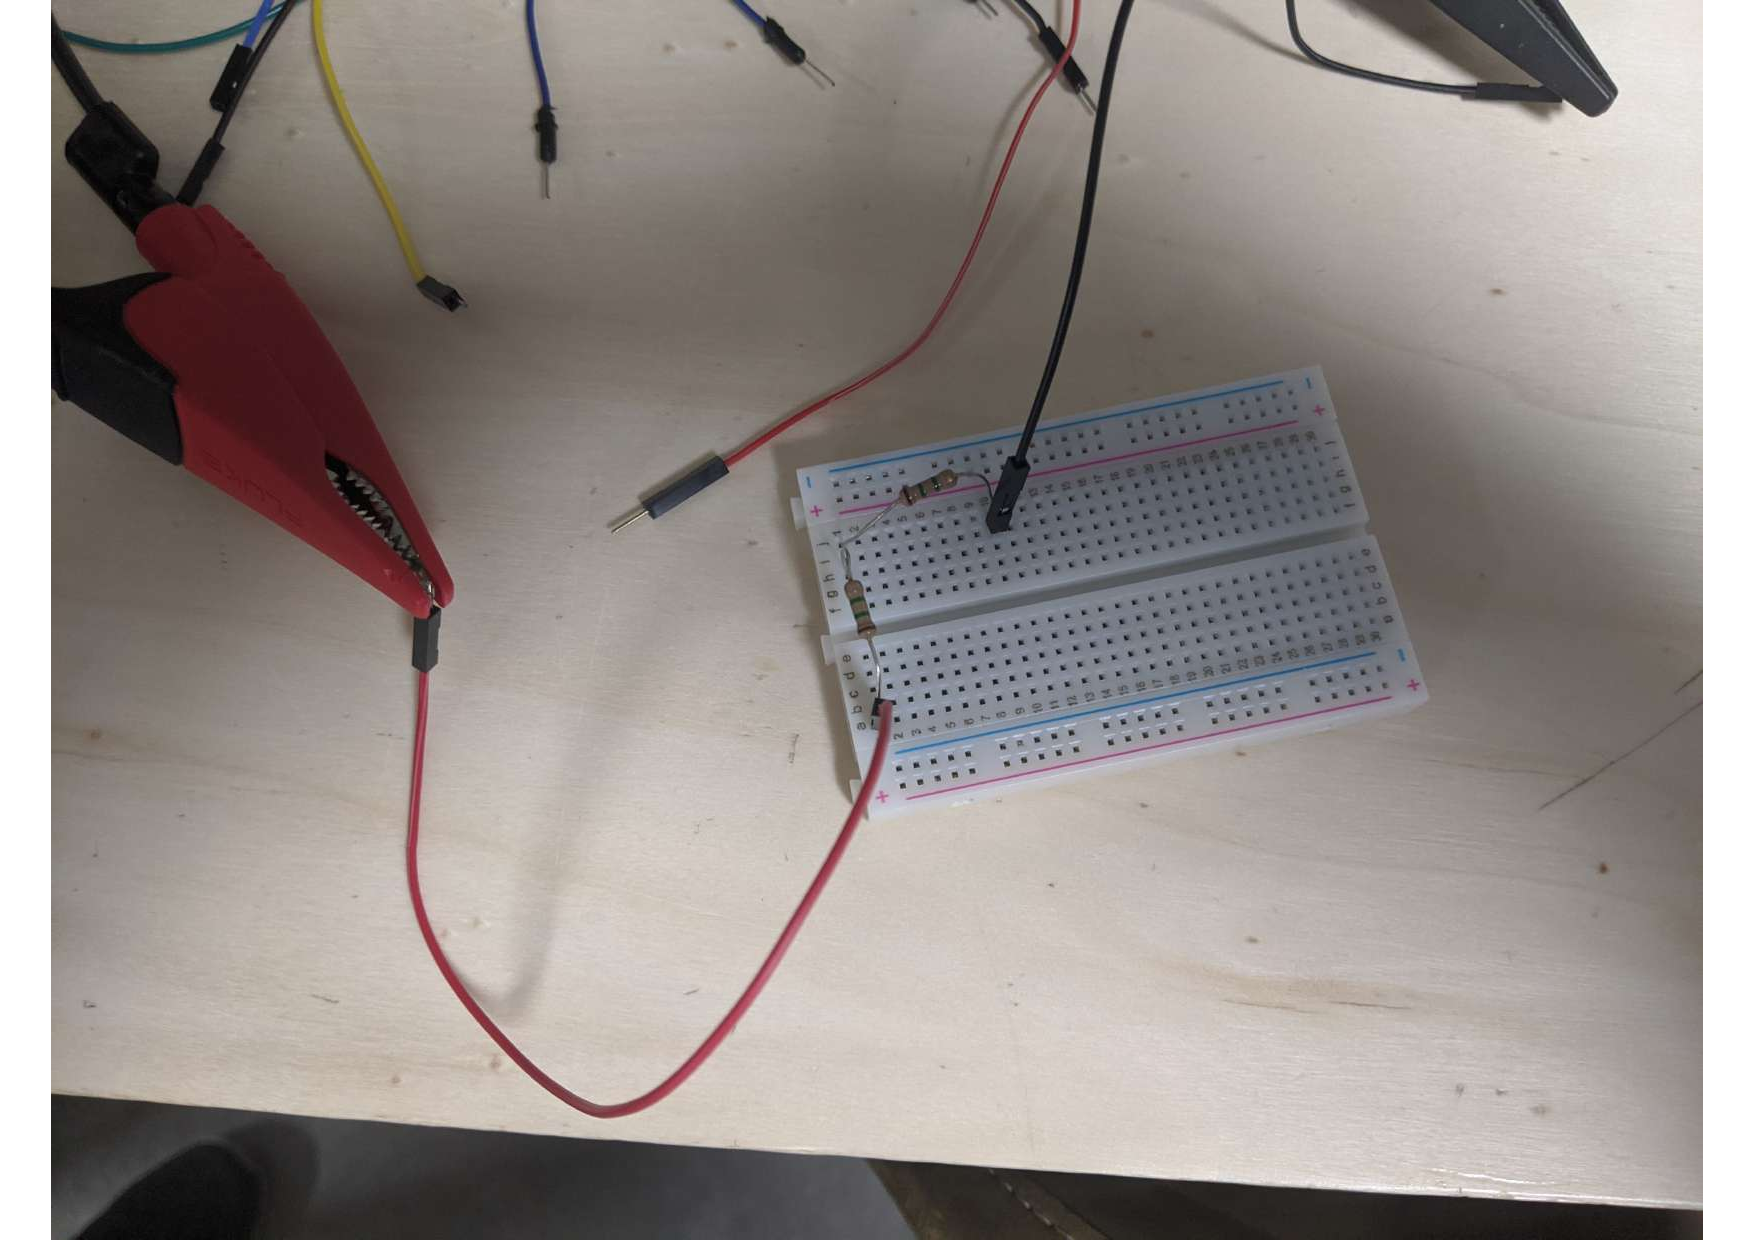
\includegraphics[width=.9\linewidth]{figures/vdc.PNG}
	\caption{Voltage divider circuit}
	\label{fig:circuit}
\end{figure}

\begin{figure}
	\centering
	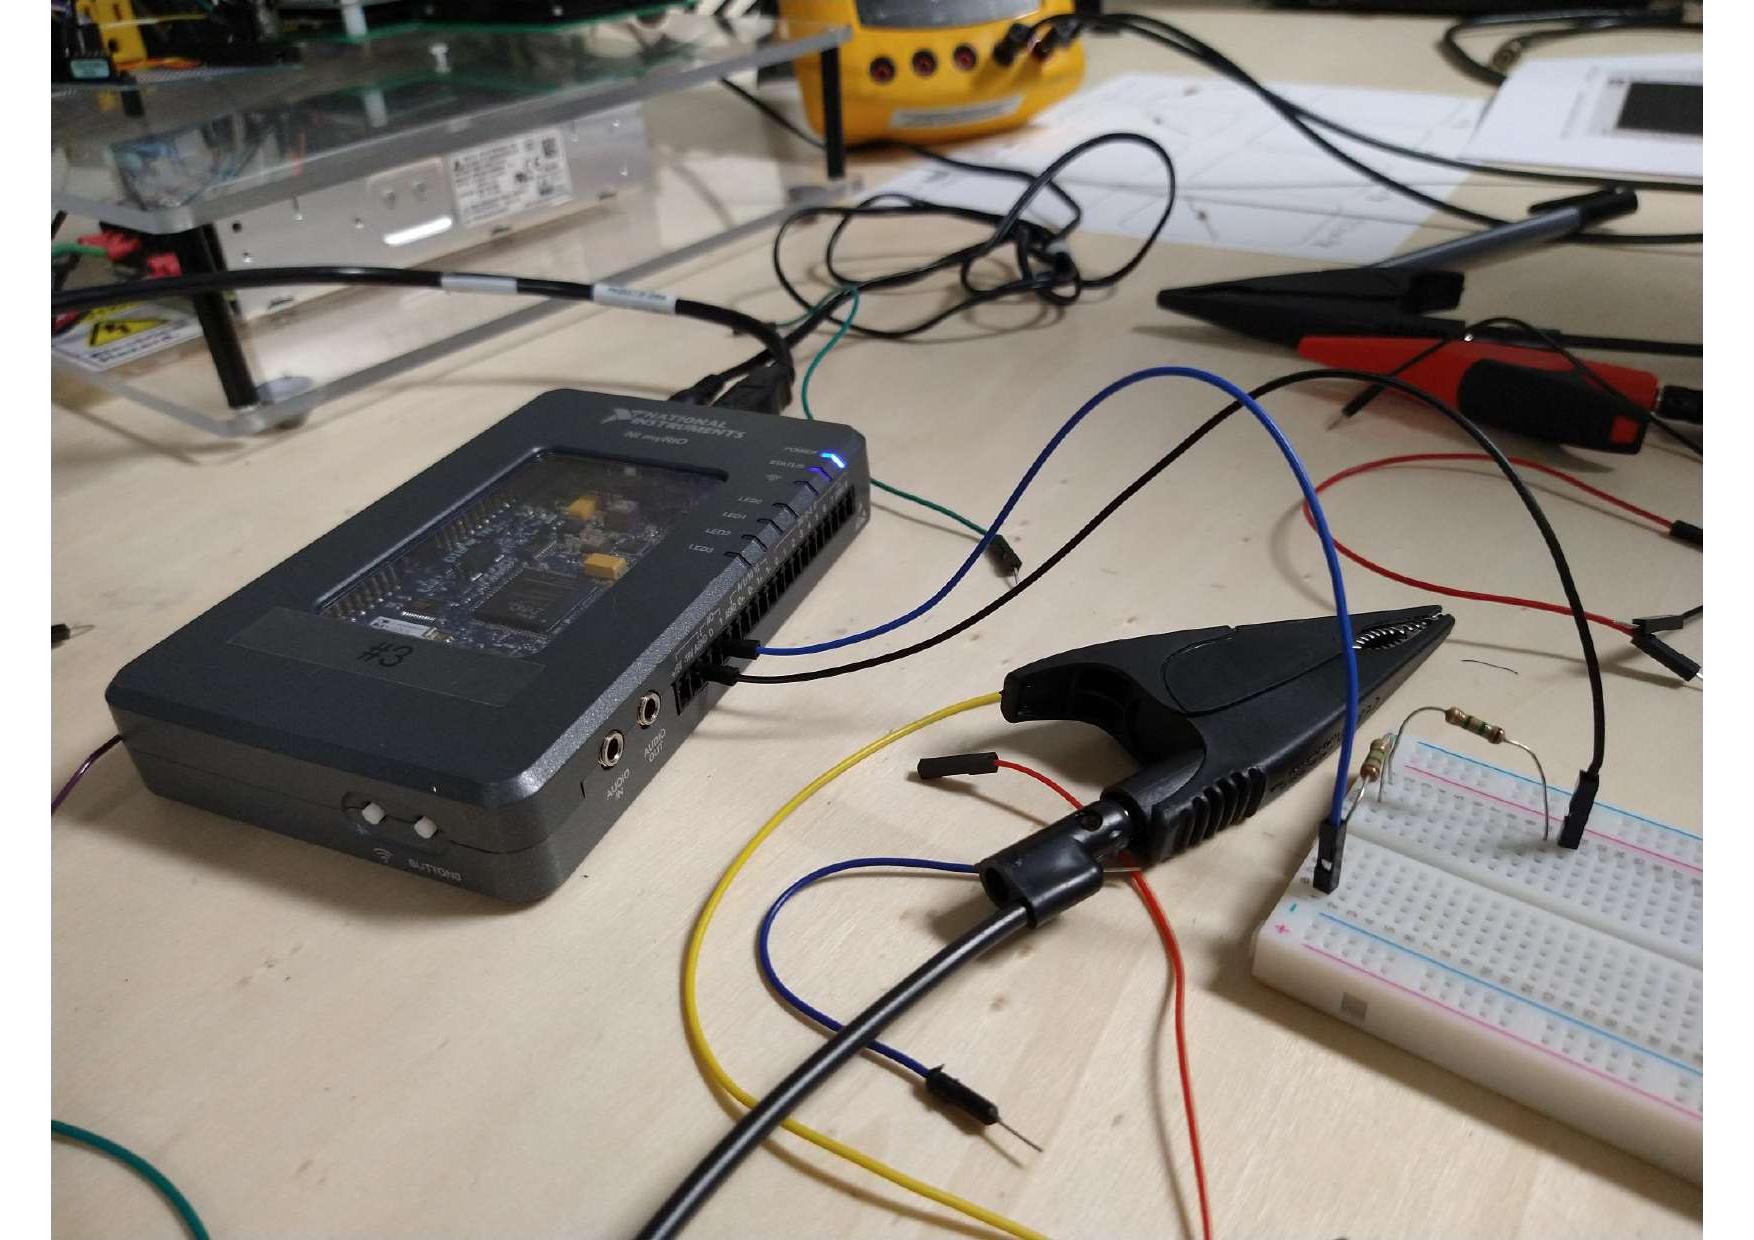
\includegraphics[width=.9\linewidth]{figures/myr.pdf}
	\caption{myRIO Ciruit}
	\label{fig:myrio}
\end{figure}

\begin{figure}
	\centering
	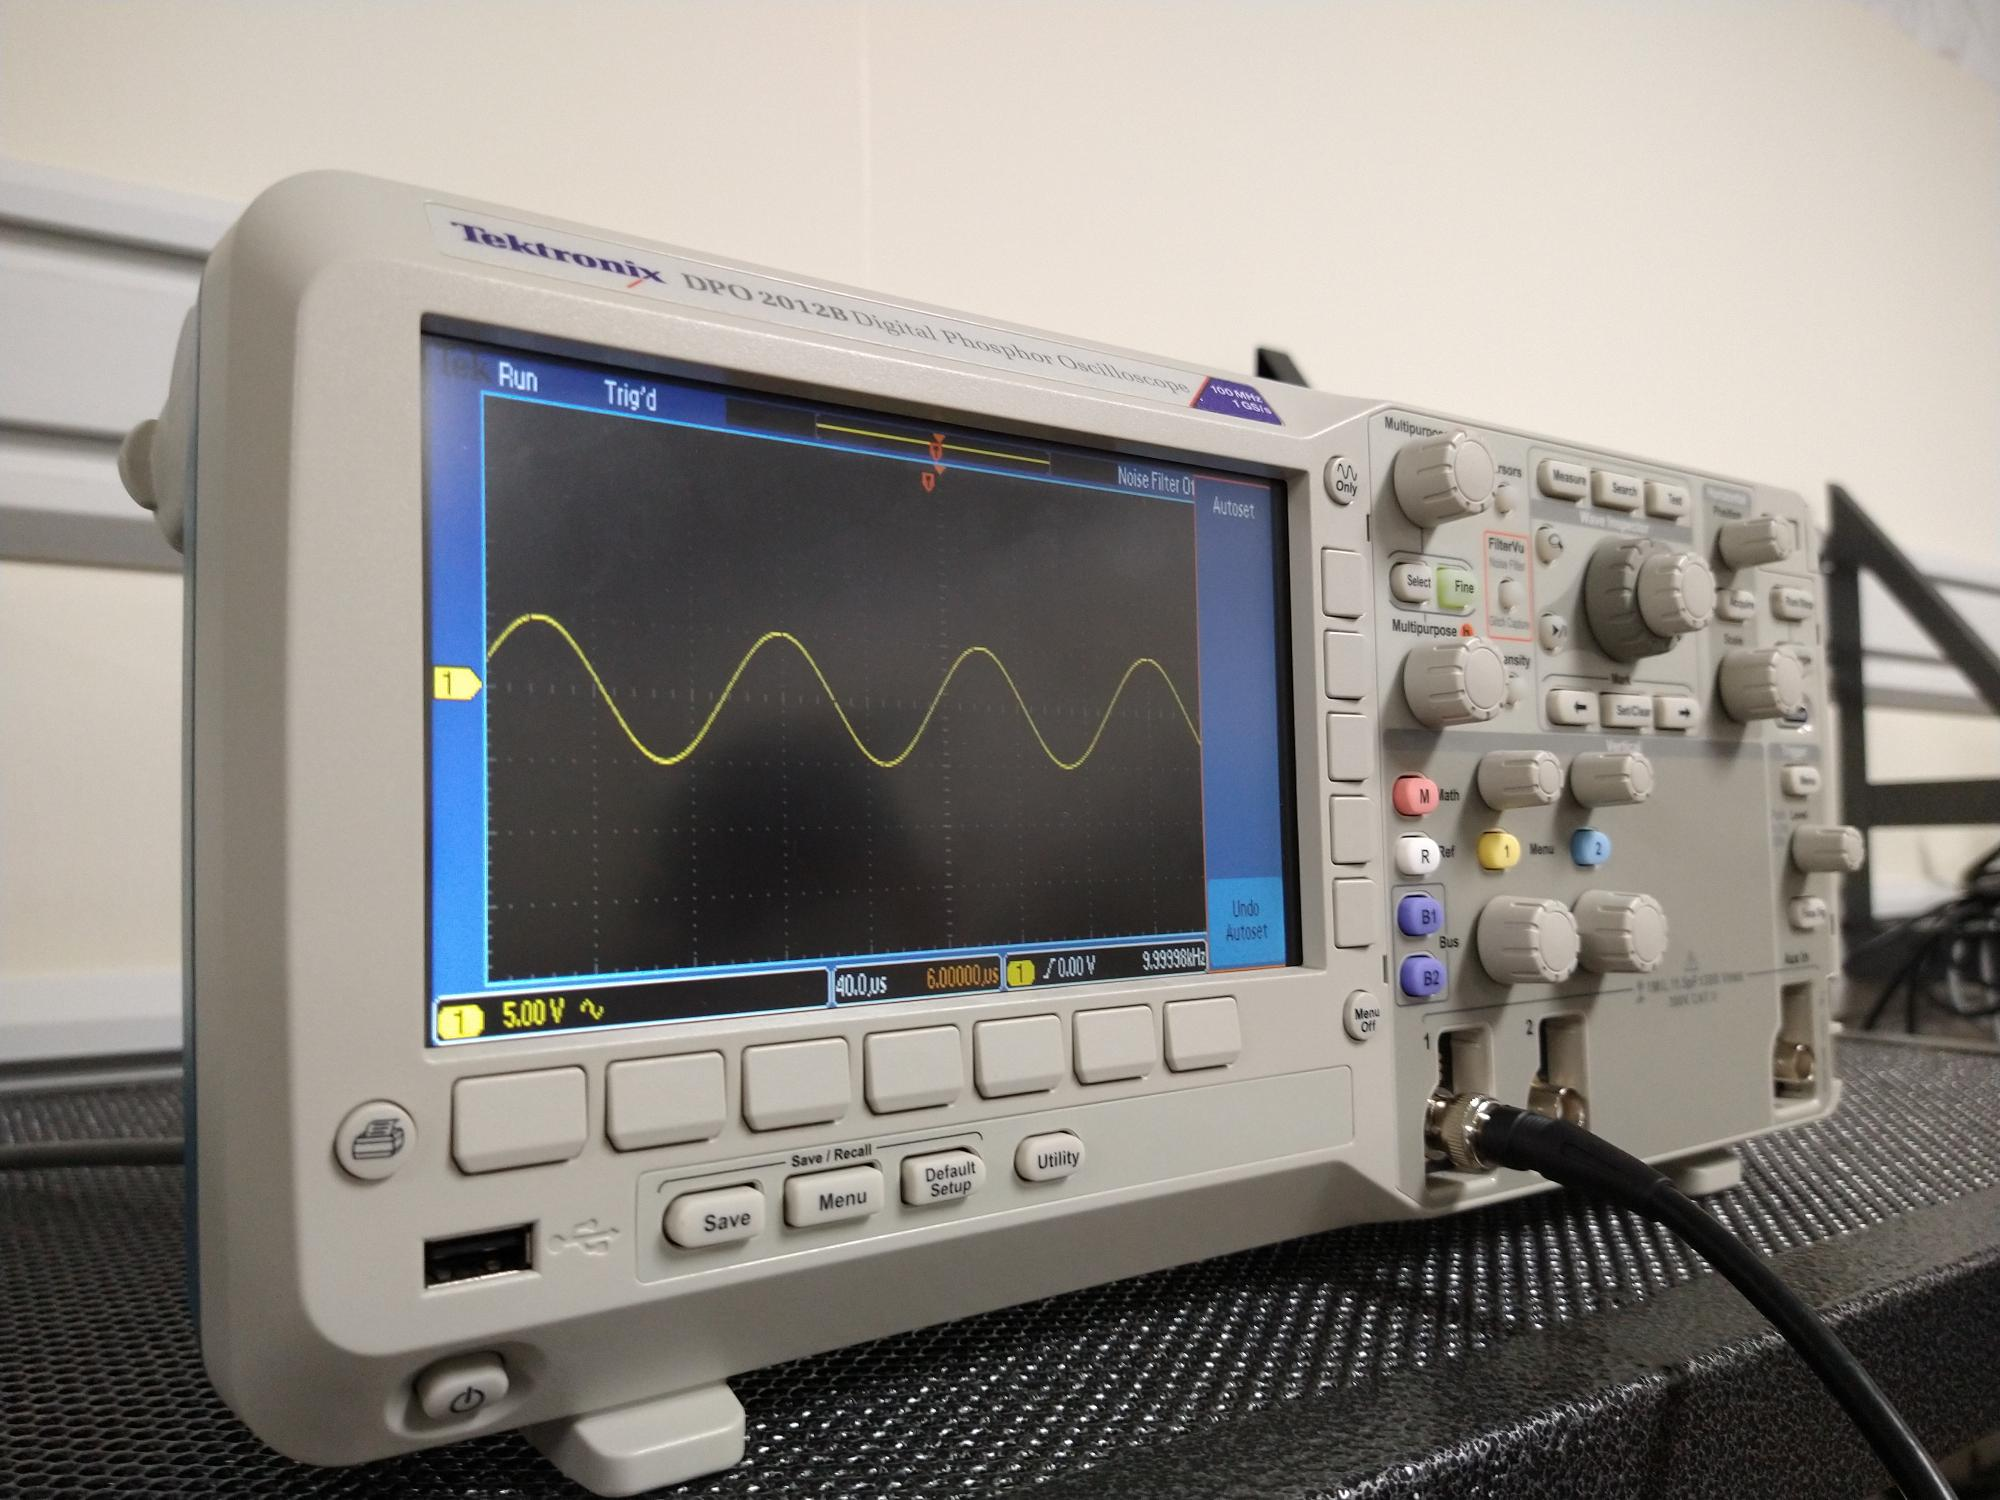
\includegraphics[width=.9\linewidth]{figures/Oscilloscope.PNG}
	\caption{Oscilloscope}
	\label{fig:stable}
\end{figure}


\section{Results}

 In the first section of the lab the results showed that as the total resistance changed for the circuit the total voltage across the circuit was not changing. The voltage across the second resistor changed when the resistance changed. \autoref{tab:Tab1}
 
 	After connecting the myRIO to the circuit and proceeding through the different input voltages we found that, again, the voltage through the entire circuit was constant no matter the total resistance and the voltage through the resistor depended on the amount of resistance.\autoref{tab:Tab2}
 	
 	When observing the stable wave made by the function generator in the oscilloscope it was estimated that the peak-peak amplitude was a 5V with a period of 2.5ms. Even when changing the shape of the wave the period and amplitude stayed the same.  
 	  
\section{Equations}


	\begin{equation}\label{eq:1}
		 V=iR
	\end{equation}
\\
	\begin{equation}\label{eq:2}
		\bm{V_{out}} = \bm{V_{in}}\left(\frac{R2}{R1+R2}\right)
	\end{equation}

\section{Discussion}
Above all else, this lab demonstrated the efficacy of what we learned in class lecture concerning the voltage divider equation and it made our group more familiar with the technology we will be continuously using throughout the semester and possibly in future careers. We have learned exactly what happens in a circuit that contained a voltage divider (two resistors in series with an outpot voltage that is a fraction of the input). During the initial portion of the lab when measuring voltage drops across the whole circuit vs. the resistors, we would see consistent drops of 60%-30% during the latter measurements compared to the former which saw almost no voltage drop at all. 

When using the myRIO software and pushing different source voltages through the various resistors the results were predictable and similar to the first part of the lab, with the voltages across the resistors being a fraction of the source voltage. Resistors 2 and 3 were at about a 50% voltage loss, and resistors 4 and 5 saw about a 40% drop. This further reinforces what we had learned about the properties of a voltage divider circuit. Speaking to other groups in the lab they observed the same results.

In our last section the group had trouble setting up the oscilloscope to produce a solid sine wave shape. After spending an inordinate amount of time, we were able to achieve success and estimated, as stated above in our results section, that the peak amplitude was 5V. We shifted the wave to different shapes like a square wave and this did not change. 

\begin{figure}
	\centering
	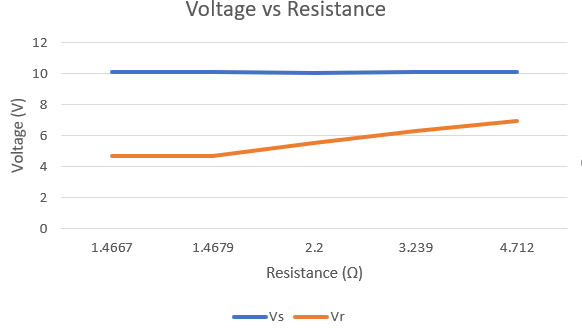
\includegraphics[width=.9\linewidth]{figures/V vs R.PNG}
	\caption{}
	\label{fig:graph}
\end{figure}

\begin{figure}
	\centering
	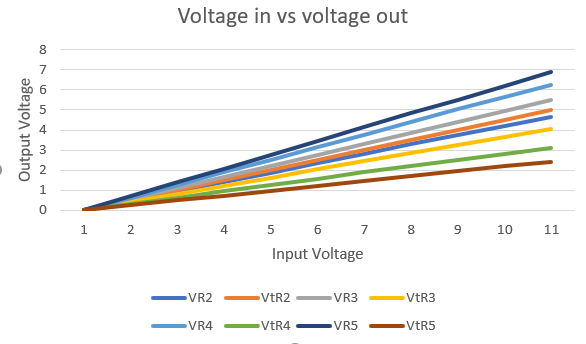
\includegraphics[width=.9\linewidth]{figures/Vin vs Vout.PNG}
	\caption{Vin vs Vout(Measured and Theoretical)}
	\label{fig:vin/out}
\end{figure}

\section{Author Contributions}

In this lab report, Austin created the figures and tables that were used as a visual representation of the data as well as several of the sections including the abstract, materials and methods, and results.
The photographs were taken by Irfan and Alex during the experiment and they combined for the rest of the report including the introduction, discussion, and this very contributions section. Editing was a team effort in order to catch each other's mistakes and make the overall report as readable and professional as possible. 

\begin{table}
	\begin{tabularx}{1\linewidth}{ lXXXXX|cXXX }
		\hline
		 & \textbf{R1} & \textbf{R2} & \textbf{R3} & \textbf{R4} & \textbf{R5}\\
		\hline
		Ri(MΩ) & 1.4667 & 1.4679 & 2.2 & 3.239 & 4.712 \\
		\cline{1-6}
		Vs(V) & 10.093 & 10.093 & 10.091 & 10.093 & 10.097 \\
		\cline{1-6}
		Vr(V) & 4.691 & 4.708 & 5.547 & 6.321 & 6.936 \\
		\hline
	\end{tabularx}
	\caption{Multimeter measurments.}
	\label{tab:Tab1}
\end{table}

\begin{table}
	\begin{tabularx}{1\linewidth}{ lXXXXX|cXXXXXXXXXXXXXXXXXXXX }
		\hline
		 & \textbf{nom. Vs} & \textbf{R2} & \textbf{R3} & \textbf{R4} & \textbf{R5}\\
		\hline
		Vs(V) & 0 & 0.006 & 0.006 & 0.006 & 0.006 \\
		Vr(V) & 0 & 0.002 & 0.003 & 0.003 & 0.004 \\
		\cline{1-6}
		Vs(V) & 1 & 1.0101 & 1.010 & 1.010 & 1.010 \\
		Vr(V) & 1 & 0.471 & 0.555 & 0.632 & 0.693 \\
		\cline{1-6}
		Vs(V) & 2 & 2.015 & 2.015 & 2.015 & 2.015 \\
		Vr(V) & 2 & 0.940 & 1.107 & 1.241 & 1.384 \\
		\cline{1-6}
		Vs(V) & 3 & 3.013 & 3.013 & 3.013 & 3.013 \\
		Vr(V) & 3 & 1.406 & 1.656 & 1.887 & 2.070 \\
		\cline{1-6}
		Vs(V) & 4 & 4.018 & 4.018 & 4.018 & 4.018 \\
		Vr(V) & 4 & 1.875 & 2.209 & 2.516 & 2.760 \\
		\cline{1-6}
		Vs(V) & 5 & 5.023 & 5.023 & 5.023 & 5.023 \\
		Vr(V) & 5 & 2.344 & 2.761 & 3.145 & 3.450 \\
		\cline{1-6}
		Vs(V) & 6 & 6.027 & 6.027 & 6.027 & 6.027 \\
		Vr(V) & 6 & 2.813 & 3.313 & 3.774 & 4.140 \\
		\cline{1-6}
		Vs(V) & 7 & 7.032 & 7.032 & 7.032 & 7.032 \\
		Vr(V) & 7 & 3.282 & 3.866 & 4.403 & 4.830 \\
		\cline{1-6}
		Vs(V) & 8 & 8.030 & 8.030 & 8.030 & 8.030 \\
		Vr(V) & 8 & 3.748 & 4.415 & 5.028 & 5.516 \\
		\cline{1-6}
		Vs(V) & 9 & 9.035 & 9.035 & 9.035 & 9.035 \\
		Vr(V) & 9 & 4.218 & 4.967 & 5.658 & 6.207 \\
		\cline{1-6}
		Vs(V) & 10 & 10.011 & 10.011 & 10.011 & 10.011 \\
		Vr(V) & 10 & 4.673 & 5.504 & 6.269 & 6.877 \\
		\hline
	\end{tabularx}
	\caption{myRIO w/ labVIEW read outs.}
	\label{tab:Tab2}
\end{table}

\end{document}  
